\documentclass[10pt,a4paper]{article}
\usepackage[utf8]{inputenc}
\usepackage[english]{babel}
\usepackage{amsmath}
\usepackage{amsfonts}
\usepackage{hyperref}
\usepackage{amssymb}
\usepackage{graphicx}
\usepackage{xcolor}
\usepackage{pdfpages}
\usepackage{listings}
\lstset{basicstyle=\ttfamily,
  showstringspaces=false,
  commentstyle=\color{red},
  keywordstyle=\color{blue}
}
\usepackage[left=2cm,right=2cm,top=2cm,bottom=2cm]{geometry}
\author{Henry Hoegelow}
\title{ePC NonLinux}
\begin{document}
\maketitle
\section{Abstract}
The C15 has a built-in embedded PC used for synthesizing the audio of the instrument. So far, the so called ePC used to run on Windows. The "Emphase" ensemble running on Native Instruments Reaktor did the audio synthesis.\\
To have less licensing costs, better performance and more control, we decided to reimplement the synthesis engine in pure C++ and to replace the operating system with a linux. This article explains, how the linux os (from now on: NonLinux) is generated, installed and updated.

\section{Basic Decisions}
The NonLinux has to be rock solid, as the OS has no human interface devices connected. Thus, if there are any problems that require user input (e.g. tweaking the BIOS, booting from USB etc), we have to pick up the device, open the housing, repair the ePC, ship it to the customer again. To avoid this costy process, we came up with a bunch of decisions and scripts, which are explained here briefly:
\subsection{Partitioning}
The internal SSD is partitioned into 4 parts:
\begin{enumerate}
\item sda1: The EFI boot partition\\
This partition contains the boot loader, the initramfs and two hooks:
\begin{itemize}
\item oroot:
The oroot hook does the setup of the later root filesystem. Therefor, it creates an overlay stack of sda2, sda3/os-overlay and sda3/runtime-overlay. The reason for this is explained later.
\item nlhook:
The nlhook tries to download a "update.tar" either from network (192.168.10.11:80/update.tar - we expect the BeagleBoneBlack to be reachable at this IP address) or from the root folder of any connected USB stick.\\
On successful download, the update.tar is unpacked. It should contain one of the following two files:
\begin{itemize}
\item backdoor.sh\\
If this file exists, it will simply be started. We can implement any update, rescue or modification logic in here. Of course, the backdoor has to be handled with care, as \begin{quote}"With great power goes great responsible."\end{quote}
\item NonLinuxOverlay.tar.gz\\
If this file is found in the update.tar, it will simply replace the contents of sda3/os-overlay. With this simple mechanism, we can update the underlying factory os by overlaying it with new contents. This includes removal of files, links, libraries, binaries etc.
\end{itemize}
Both files, backdoor.sh and NonLinuxOverlay.tar.gz are only accepted by the update process, if there exists a file with the SHA-256 sum of the according file at the same filesystem level. So, if the SHA-256 sum of backdoor.sh is "1234567890", the update script expects a file named "1234567890.sign" to exist.
\end{itemize}
\item sda2: The factory NonLinux\\
This partition contains a full working NonLinux. The C15 should be able to boot this OS and provide basic functionality.
\item sda3: The overlays\\
On the sda3 partition, there are two important folders: 
\begin{itemize}
\item os-overlay:\\
This folder contains the difference between the factory os in sda2 and the updated os that the C15 actually boots. Our updates are copied here.
\item runtime-overlay:\\
All changes to the file system done later by running processes, are kept here. The folder is cleared on every boot - so all changes done in a booted system are reverted with a reboot.
\end{itemize}
\item sda4: Home\\
This partition is for storing user generated stuff, like settings and presets.
\end{enumerate}

\begin{center}
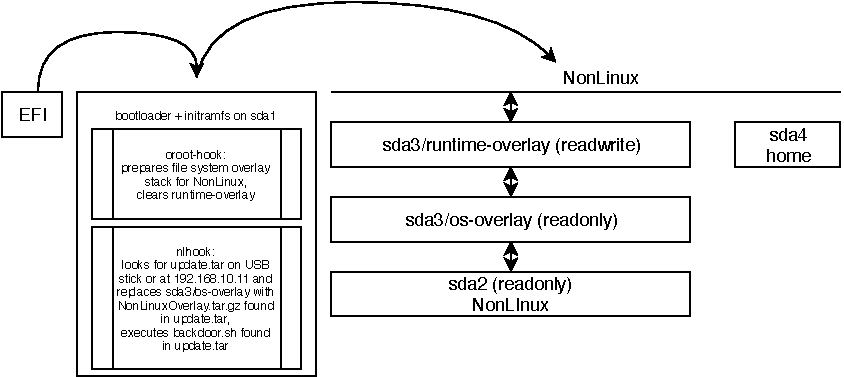
\includegraphics[scale=1.0]{ePC.pdf}	
\end{center}

\subsection{Linux Distribution}
After doing some performance tests, we decided for Audiophile Linux as base for our NonLinux. Audiophiophile Linux in turn is based on Arch Linux, which is a very flexible and lightweight distribution. On the other hand, Arch Linux is a distribution for the experienced user, as it comes without graphical configuration tools and most of the steps for installation and configuration has to be done manually.\\
Audiophile Linux uses the linux realtime kernel patch to enable preemptive thread scheduling yielding more reliable performance results.\\

\subsection{Audiophile2NonLinux repository}
We maintain a github repository at \url{https://github.com/nonlinear-labs-dev/Audiophile2NonLinux}. It contains all scripts and modifications done to Audiophile Linux to turn it into a NonLinux. 

\section{NonLinux Installation}
\subsection{On a NUC}
To install NonLinux an a NUC, you have to perform the following steps:
\begin{enumerate}
\item Download the Audiophile Linux ISO image from \url{https://sourceforge.net/projects/ap-linux/}
\item Create a bootable USB stick containing the downloaded image.
\item Connect monitor, keyboard and ethernet to the NUC.
\item Tweak the BIOS to enable UEFI boot.
\item Boot the AP Linux from USB stick.
\item type:
\begin{lstlisting}[language=bash,breaklines=true]
curl -L "https://github.com/nonlinear-labs-dev/Audiophile2NonLinux/raw/master/runme.sh" | sh
\end{lstlisting}
\end{enumerate}
The system will now be configured by the downloaded script.\\
The most time consuming part of the script is the download of the NonLinux.pkg.tar.gz package repository. In order to speed up the download, the script will test several location for faster download. Currently, it tries to download from
\begin{itemize}
\item http://192.168.2.180:8000 (my, hhos, development PC)
\item http://192.168.0.2:8000 (The Buildservers internal IP)
\item http://185.28.186.202:8000 (The Buildservers external IP)
\item https://github.com/nonlinear-labs-dev/Audiophile2NonLinux/releases/download/1.0
\end{itemize}
Thus, the download can be speed up by starting a local http server, serving the NonLinux.pkg.tar.gz file:
\begin{lstlisting}[language=bash,breaklines=true]
python -m SimpleHTTPServer /path/to/folder/containing-NonLinux-package-repository
\end{lstlisting}
\subsection{On a VM}
\label{vm-install}
Basically, the steps above can be easily adapted to install NonLinux in a VM. Still, setting up the VM and typing the URL is error prone and avoidable. So, I implemented a script that can be run on a development pc like this:
\begin{lstlisting}[language=bash,breaklines=true]
# in the git folder of the Audiophile2NonLinux project:
./run-me-on-vm-host.sh /folder/containing/the/AudiophileLinux-ISO-image
\end{lstlisting}
The script will create, start and setup a virtual machine, finally containing a factory NonLinux.
This VM can be used for testing or as origin for creating updates.
\section{Updates}
As described earlier, updates are delivered as content for the sda3/os-overlay folder or as backdoor.sh.
The backdoor.sh has any freedom to heal or damage the system and should be used only in emergency cases.\\
The NonLinuxOverlay.tar.gz is meant to contain all files, links and removals neccessary to turn a factory NonLinux into the updated NonLinux. Note, that this process is NOT meant to be incremental. If Update2 relies on files shipped with Update1, it has to contain the according files, too.\\
\subsection{How to create an update}
\begin{itemize}
\item Start a new VM as explained in \ref{vm-install}.
\item Tweak the OS as you like, you can
\begin{itemize}
\item Add/remove/move files
\item install binaries
\item set or remove links
\item start or disable system services
\end{itemize}
If the system is set up properly, call 
\begin{lstlisting}[language=bash,breaklines=true]
/createUpdateFromRunningOS.sh
\end{lstlisting}
in the root folder. This will provide you the file "/update.tar". You can push this to a computer in the network by calling
\begin{lstlisting}[language=bash,breaklines=true]
scp /update.tar user@machine:
\end{lstlisting}
\end{itemize}

\section{Todo}
There are still some issues left:
\begin{itemize}
\item Playground has to offer the update.tar, if a stick is connected to BBB.
\item Updating a Windows or Win/Linux machine from BBB over ssh is not yet tested.
\item Even though the nlhook waits up to 3 seconds on downloading the update.tar from BBB, it experiences a "wget timeout" from time to time.

\end{itemize}
\end{document}